\section{Durchführung}
\label{sec:Durchführung}

In Abbildung \ref{fig:aufbau} ist der Aufbau des Versuchs zu sehen.

\begin{figure}
    \centering
    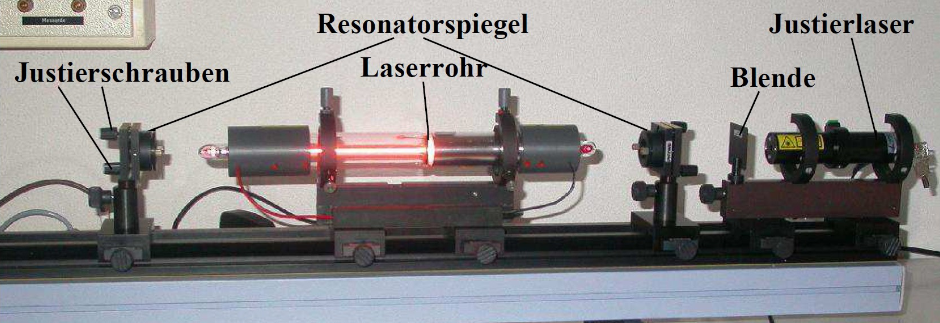
\includegraphics[width=\textwidth]{data/aufbau.png}
    \caption{Aufabu mit wesentlichen Komponenten}
\end{figure}

Für einen stabilen Laserstrahl ist die vorherige Justierung unabdinglich.
Mit Hilfe des Justierungslasers werden die Spiegel so eingetsellt, dass der Laserstrahl mittig auf die Blende zurückfällt.
Während der eigentlichen Messung ist der Justierungslaser ausgeschaltet.\\
Als erstes soll die Stabilitätsbedingung überprüft werden. 
Dazu wird eine Messreihe der Lichtintensität in Abhängigkeit von der Resonatorlänge mit einer Photodiode, welche die Intensität als Strom ausgibt, durchgeführt.
Es werden zwei konkave Spiegel mit Krümmungsradius von $r_i=1,4\,$m genutzt.
Während des Verschiebens der Spiegel ist eine Nechjustierung notwendig um den Laserstrahl mit maximaler Leistung aufrech zu erhalten.\\
Gleichzeitig wird die Schwebungsfrequenz vermessen.
Dazu wird mit dem Spektrumanalysator jeweils das Fourierspektrum zur Resonatorlänge aufgenommen.\\

Danach werden die transversalen Moden untersucht.
Durch eine Streulinse auf der optischen Schiene wird der aufgefächerte Laserstrahl auf die Photodiode projeziert.
Die mit einer Skala versehene Diode kann nun die Intensitätsverteilung entlang der $x-$Achse aufnehmen.
Weil die TEM$_{0,0}$ Mode das Spektrum dominiert kann diese ohne weiteres vermessen werden.
Für die TEM$_{1,0}$ und TEM$_{2,0}$ Moden wird die Stellung des Laserrohrs leicht verfälscht um diese sichtbar zu machen.\\

Im dritten Teil des Versuchs soll die Polarisation des Laserstrahls untersucht werden.
Dazu wird ein Polarisationsfilter von $0$ bis $180\circ$ im Strahlengang variiert und dahinter die Intensität gemessen.\\

Zuletzt soll die Wellenlänge durch Beugung an einem Gitter berechnet werden.
Der Schirm, auf den projeziert wird, wird mit großem Abstand zum Gitter aufgestellt.
Für eine höhere Genauigkeit wird der Abstand soweit erhöt, dass nur noch das nullte und jeweils erste Maximum auf jeder Seite sichtbar ist.
Der Abstand der beiden ersten Maxima vom nullten Maximum, der Abstand von Gitter und Schirm, sowie die Gitterkonstante wird für zwei Verschiedene Gitter aufgeschrieben.